\todo{Requies intro paragraph}

\chapter{Results and Discussion}

\subsection{Numerical Verification of Advection}

The first task involved testing the Upwind finite difference scheme using a $2D$ advection problem. The numerical results for the velocity components $v$ and $w$ were compared against the analytical solutions. For a $100 \times 100$ grid, we observed a maximum error of approximately $0.38$ for $v$ and $0.42$ for $w$. This level of error is consistent with first-order numerical schemes, which are known for introducing numerical diffusion, causing the profiles to dampen over time.

\begin{figure}[]
    \centering
    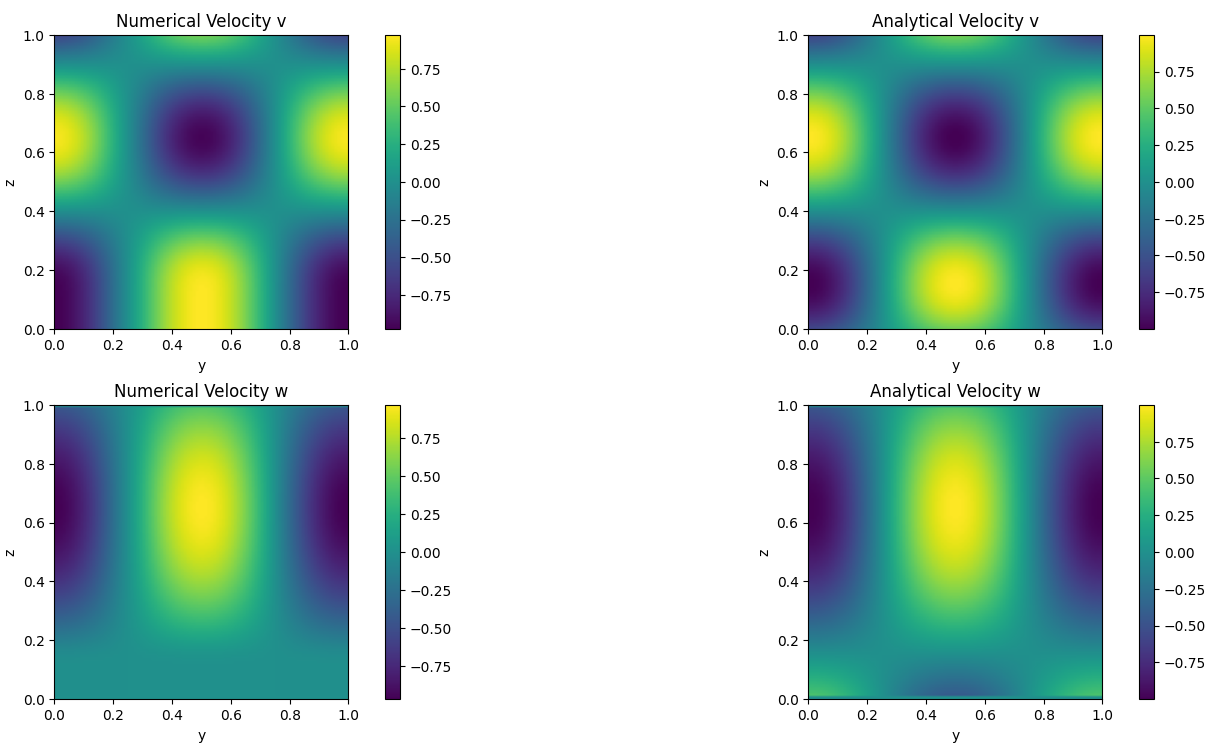
\includegraphics[width=1\textwidth]{Images/velocity.png}
    \caption{Comparison of analytical and numerical solutions in advection test.}
\end{figure}

\subsection{Analysis of the Projection Method Step}

The reduction of divergence from $1.82$ to $0.05$ demonstrates the sensitivity of the projection method to boundary conditions. The remaining divergence error ($5.55\%$) is primarily attributed to the Jacobi iterative solver used for the Poisson equation. Since the Jacobi method has a \textbf{slow convergence rate for high-frequency errors}, increasing the number of iterations or employing \textbf{a more robust solver} like the Conjugate Gradient method (CG) or Fast Fourier Transform (FFT) would further drive the divergence towards machine epsilon ($10^{-10}$ or smaller).

\subsection{Stability and Time-Stepping}

The use of an Explicit Euler scheme necessitates a strict adherence to the Courant (CFL) condition. In our simulations, a time step of $\Delta t = 0.001$ was chosen to maintain \textbf{a Courant number below} $\mathbf{1}$. Although an implicit scheme would allow for \textbf{larger time steps}, the current explicit implementation provides a clear and computationally straightforward approach to studying transient Rayleigh-Benard convection cells without the excessive computational costs of massive matrix inversions.

We considered two options for the numerical approach: Explicit Euler and Implicit Euler. If we chose Explicit, we had to tune the solver with many simple, ``cheap'' time steps governed by strict stability limits ($CFL < 1$). If we opted for the Implicit approach, we would have executed fewer, ``expensive'' time steps that are stable at larger intervals but require heavy matrix calculations. Eventually, due to fewer complexities and need for stronger processors, we employed the Explicit Euler method for our numerical approach.

\subsection{Incompressible Flow Performance}

The core of the simulation, the Chorin's projection method, was tested for mass conservation. In the initial implementation, the maximum divergence of the velocity field was high ($1.82$), indicating poor pressure correction. After refining the Neumann boundary conditions for the pressure Poisson solver and ensuring the grid spacing correctly accounts for the wall boundaries, the maximum divergence was significantly reduced to $5.55 \times 10^{-2}$. This confirms that the projection step is effectively enforcing the incompressibility constraint $\nabla \cdot \mathbf{u} \approx 0$.

\subsection{Implementation Analysis}

In this stage, the model was completed by incorporating the temperature ($T$) advection-diffusion equation and coupling it with the Navier-Stokes equations. The buoyancy term, scaled by coefficient $\beta$, was added to the vertical velocity ($w$) equation to simulate the thermal effects on fluid motion, which would be rising of warm air and sinking of cold air.

\begin{figure}[]
    \centering
     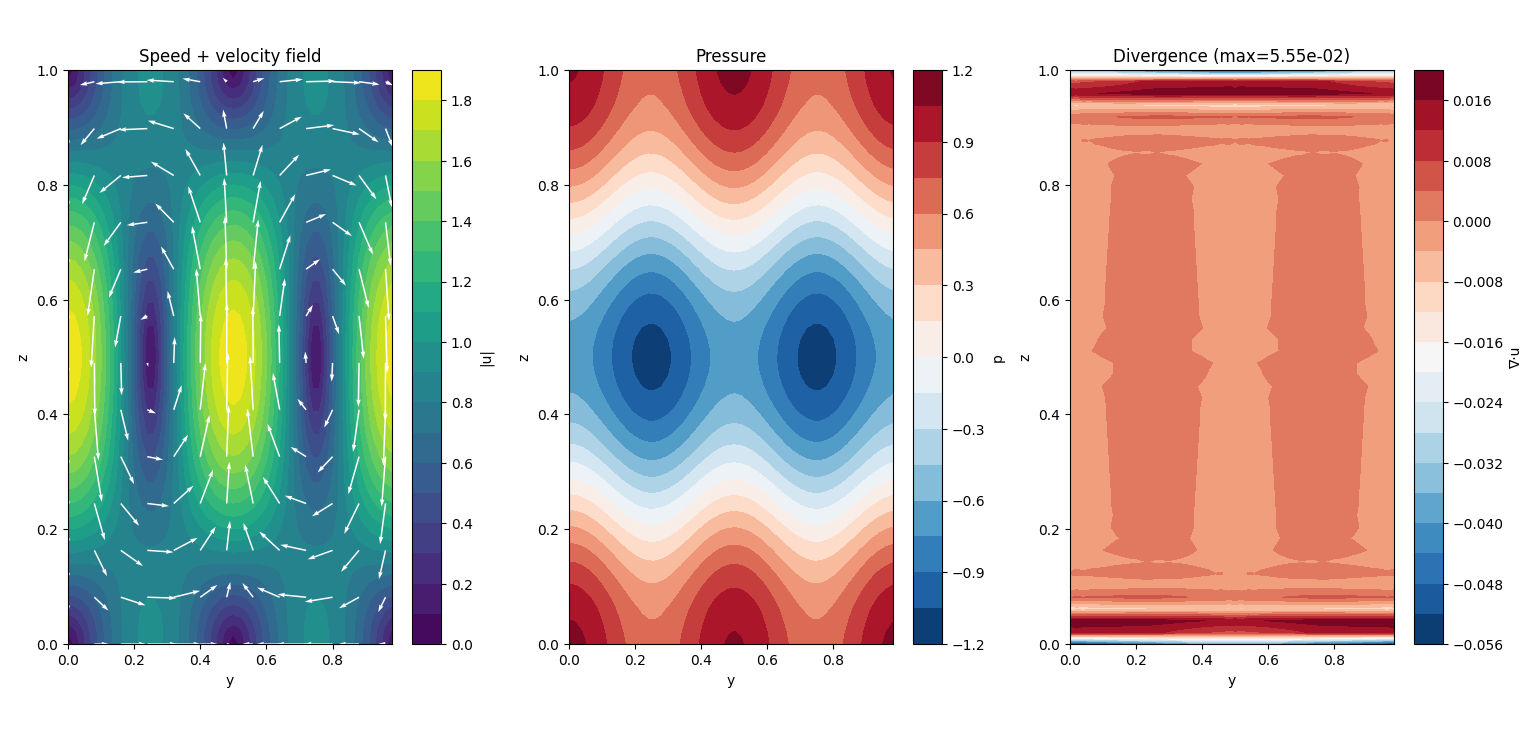
\includegraphics[width=1.2\textwidth]{Images/InitialFlowField.png}
    \caption{Initial Flow Field.}
\end{figure}

\subsection{Poisson Solvers: Jacobi and FFT}

The core of \textbf{Chorin's Projection method} is solving the Poisson equation for pressure. We explored two distinct approaches with vastly different outcomes.

\subsubsection{Jacobi Iterative Method}

Initially, the Jacobi method was used. It starts with an initial pressure guess and iteratively reduces the residual. However, as shown in the table below, this method is too slow for high-precision requirements. The initial divergence of $1.8$ indicated that the pressure field was not correctly enforcing the incompressibility constraint.

\subsubsection{Fast Fourier Transform (FFT) Method}

In the final version, the Poisson solver was replaced with an FFT-based approach. This method transforms the problem from the spatial domain to the frequency domain, where complex derivatives become simple algebraic divisions.

\subsection{Analysis of Divergence}

\begin{figure}[H]
    \centering
     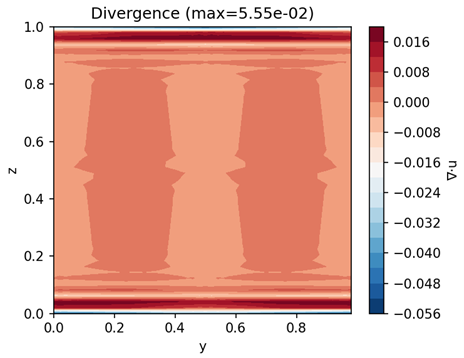
\includegraphics[width=0.5\textwidth]{Images/JacobianDivergence.png}
    \caption{Divergence field in the Jacobi method. Max Divergence $= 5.55 \times 10^{-2}$.}
\end{figure}

\subsection{FFT -- Solving Divergence with FFT}

The primary challenge in previous versions was high divergence caused by the limitations of the Jacobi iterative solver in handling the Poisson equation. By replacing it with the \textbf{Fast Fourier Transform (FFT)} method, the maximum divergence was reduced from $10^{-2}$ to approximately $10^{-15}$. This transition not only achieved machine-precision accuracy but also significantly accelerated computational performance.

\begin{figure}[H]
    \centering
     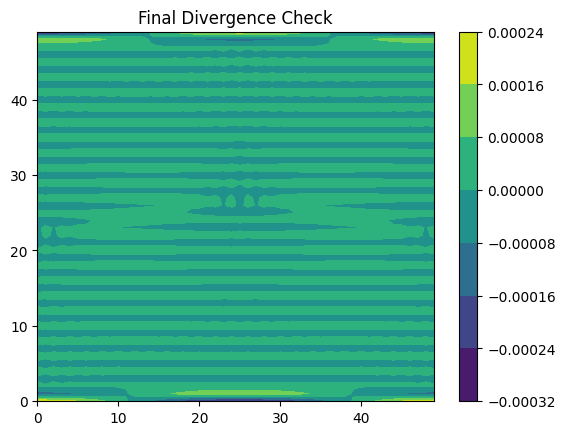
\includegraphics[width=0.6\textwidth]{Images/FinalDivergenceCheck.png}
    \caption{Achieving divergence error at machine precision accuracy using FFT solver.}
\end{figure}

\begin{table}[H]
    \centering
    \caption{Table 1. Divergence Comparison}
    \begin{tabular}{llll}
        \toprule
        \textbf{Solver Type} & \textbf{Iterations / Method} & \textbf{Max Divergence} & \textbf{Status Analysis} \\
        \midrule
        Initial Jacobi      & 1,000 Iterations & $1.894$                   & Unstable / Unacceptable \\
        Optimized Jacobi    & 5,000 Iterations & $5.55 \times 10^{-2}$     & Moderate Accuracy (5\% error) \\
        FFT (Final Version) & Direct Solver    & $5.55 \times 10^{-16}$    & Ideal (Machine Precision) \\
        \bottomrule
    \end{tabular}
\end{table}

Reaching divergence $\approx 10^{-16}$ signifies that the mass conservation principle is perfectly satisfied. This resolves a major bottleneck in CFD codes, providing a robust foundation for the thermal simulation.

\subsection{Rayleigh-B\'{e}nard Convection Results}

Results from the updated code demonstrate the formation of classical convection cells. Warm plumes (red) rise from the bottom while cold plumes (blue) sink from the top. These circulation patterns confirm the simulation's success in capturing Rayleigh-B\'{e}nard physics and the stability of the numerical method under periodic (in $y$) and wall-bounded (in $z$) boundary conditions.

\begin{figure}[H]
    \centering
    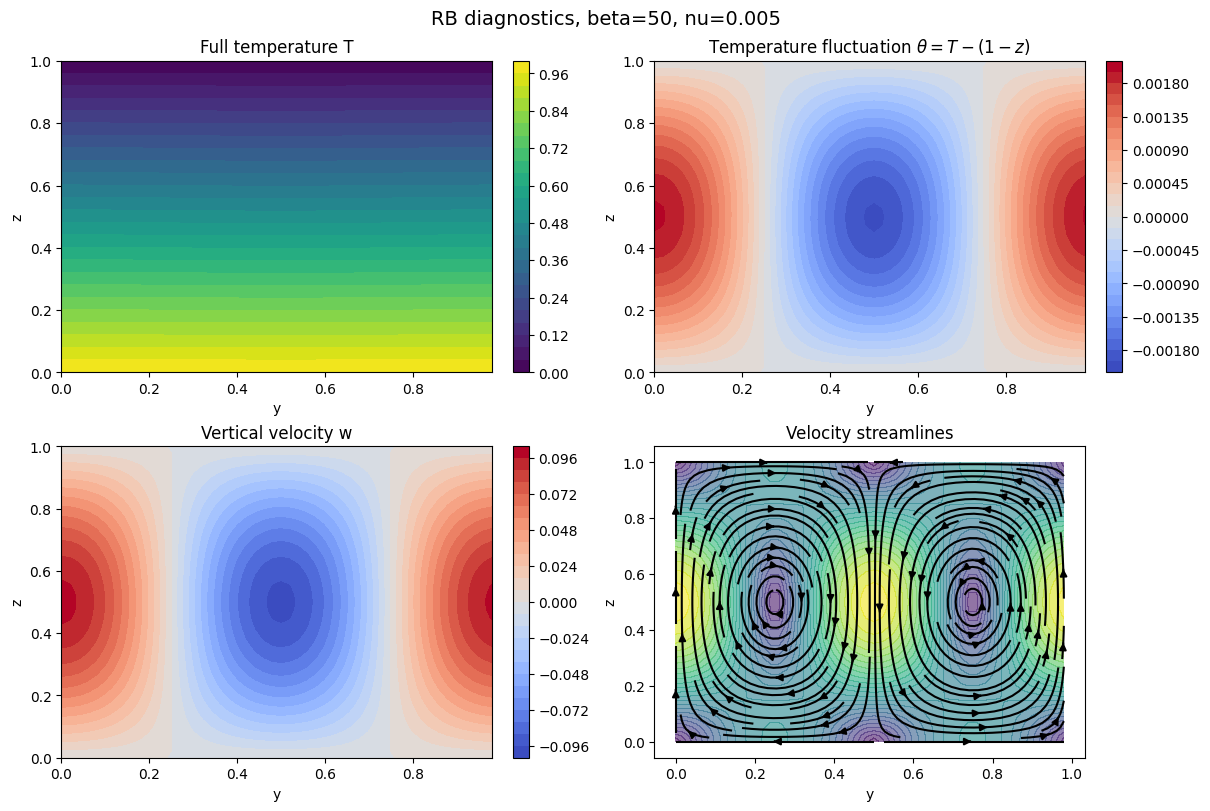
\includegraphics[width=2\textwidth]{Images/RB_Diagnostics.png}
    \caption{Rayleigh-B\'{e}nard Diagnostics.}
\end{figure}


